% This is LLNCS.DOC the documentation file of
% the LaTeX2e class from Springer-Verlag
% for Lecture Notes in Computer Science, version 2.4
\documentclass{llncs}
\usepackage{llncsdoc}
\usepackage{hyperref}
\usepackage{graphicx}
\usepackage{amsmath}
\usepackage{fixltx2e}
%
\begin{document}
%
\newpage

%
\title{A Lightweight System for Just-In-Time Aggregation of Machine Generated Data in a Distributed Network}

\author {Student: Michael Dreeling\\{ Supervisor: Eric Robson}\\{ Sept 1st 2014}}
\institute{Waterford Institute of Technology, Ireland.}

\maketitle
%
\begin{abstract}
Application Data Management or ADM is a research area concerned with the aggregation, storage and presentation of information typically emitted from Enterprise Applications. ADM is a subset of Enterprise Information Management or EIM [27]. EIM usually joins together Business Intelligence and raw Application Data. Large scale commercial EIM systems started to appear in 2003, and since then many of the larger software vendors such as Tibco, Oracle and SAP [28] have created their own systems. The goal of each system is to present the Machine Generated Data [17] or MGD being emitted from applications and servers. Over the past few years, there has been a focus in EIM on dealing with the challenge of Big-Data as companies such as Amazon, Facebook and Zynga generate terabytes of application information per day. This data, when organized, can be used in the analysis of system problems, user behavior and security threats.
\end{abstract}
%
\section{Introduction}
%
Most EIM software solutions work in either an Active, Passive or Combined operation mode. An Active system requires installation of modules or agents (sometimes called collectors) on servers which are being monitored. The agents usually run with a relatively high level of access and feed information back to a central aggregator. The agents can very efficiently pass the information back to the server and have extremely fast access to the data. A Passive system on the other hand operates entirely remotely and must work harder to retrieve and analyze the data. Typically, file and directory access will need to be granted to the host system by an Administrator over a particular protocol although software is not required to be installed once access has been granted. For the purposes of this dissertation we will focus on the Passive style. The major challenges for all EIM systems are 

\begin{enumerate}
  \item Accessing and Transmitting Data 
  \item Indexing Data
  \item Searching Data
\end{enumerate}

Data access is the most straight forward issue to solve in both the Passive and Active style as Administrators must be involved in either solution or need to at least provide some level of configuration. Data indexing and Searching however are much more difficult to solve for and as such typically involve mathematical solutions (such as Bloom Filters[22,23] for instance) to resolve. This dissertation will attempt to design a lightweight Passive analysis system which can be used to quickly aggregate and view “short term” data within a system, rather than detailed historical analysis. Such a system could be used to quickly analyze application issues during a high severity event within an Enterprise. 

This system would have several advantages over existing software

\begin{enumerate}
  \item A Light installation foot print (1 or 2 servers)
  \item Low overall CPU usage on server and monitored host
\end{enumerate}

\section{Background and related work}

In this section we will outline modern approaches to data aggregation and analysis of Machine Generated Data. This area has seen considerable innovation over the past 10 years and so there are many methods being used. Many of the systems use proprietary technology and granted patents [24]

In this section we will outline modern approaches to data aggregation and analysis of Machine Generated and JVM based Data.

\subsection{Distributed Data Collection methods}

Information from Enterprise Applications is typically stored in log files on the disks of servers running these applications. The servers may be running a variety of Unix, Linux or Windows based operating systems. 

Each server typically stores application logs in a variety of different areas on disk depending on how the application was developed. In addition to the application logs themselves, the software used to run the application may also have logs, and errors can be reported in any one of these files. Logs break down into several categories:

\begin{alpherate}
\item Be-spoke Application logs (Developer created);
\item Off-the-shelf Application Software Logs (Apache, Weblogic, Tomcat);
\item Logs generated from the RunTime Environment – for example JVM based logs (In Java environments);
\item Logs generated by the Operating system.
\end{alpherate}

In active EIM systems collection of this data is usually performed by Agents and centrally forwarded to a Log Aggregation server where it can be searched. In highly secured environments with change management concerns, a Passive approach is preferable where a centralized logging server pulls data from each server using common protocols and aggregates it afterwards.

\subsection{Active Analysis (Push)}

Compared to systems which do not require custom client software installation, Active Analysis systems typically require a large amount of setup,design and configuration, requiring Agents to be installed on the operating system which is running the monitored application. The system must then be configured to read and forward information to a central location where it is collated for presentation. Agent’s usually forward data over a network port (UDP/TCP or HTTPS) to the central aggregator. This method of collection is the very efficient as the agents have direct access to the data under analysis. This method also scales as the number of nodes under management increases. This is due to the fact that the client machines are running some of the required software, and as such the CPU usage required to retrieve the data from them is more evenly distributed.

\subsection{Passive Analysis (Pull)}

Passive Analysis systems typically require less setup and design, with more or less the same amount of configuration as Active systems. One or more central servers are installed on the network and they are configured to remotely read the logs of the monitored application. Drawbacks of this approach are that it is less efficient than having direct disk access to the files in question. The reason for this is that active analysis systems can more easily be configured to filter on certain events and feed the central server when these events occur, passive systems must analyze the data once it has been retrieved, and then decide which data to keep. Also, as it uses existing operating system software (such as SSH) to make connections to remote machines, it is also highly dependent on the operating system under analysis.

%
\subsection{Machine Generated Data}
This article [10], created relatively recently (Dec 2010) describes machine generated data as information “automatically created from a computer process, application, or other machine without the intervention of a human”. This statement is of course partially true, and is acknowledged as such, due to the fact that information generated by processes or machines is inherently tied to the humans which are interacting with it or issuing commands to the system.

It is more accurately described by Monash [17], in a provisional definition, as information “that was produced entirely by machines OR data that is more about observing humans than recording their choices”. The article goes on to further describe the categories under which MGD falls, such as the output of network, telemetry and other computer equipment appliances.

The text also categorizes MGD as information which can be, and probably should be, frequently discarded. This statement fits with the purpose of this dissertation, which is to develop a method to quickly review, but not store MGD in a “sliding window” fashion.
%
\subsection{Available Data Collection and Aggregation Systems}
GrayLog2 [1] is an open sourced centralized logging system intended for use by organizations’ in order to provide a window onto real-time and historical log data. The data is pushed to Graylog’s server (graylog-server) using syslog from each registered node in data pipelines known as ‘streams’. The nodes themselves must be registered within GrayLog using its UI interface. Gray log records the Date, Host, and Level of each of the incoming messages. It reports the number of message per second which are coming into the system in the UI. It has advanced searching features using Elastic Search as it’s backend, which even allows some natural language to be used when searching records (i.e you can search a Timeframe such as ‘from yesterday’). This UI also provides advanced graphing and tracking of multiple sources at once. It does not support a centralized Multi-SSH server siphon as outlined in the dissertation.

LogStash [5] is also an open sourced tool for managing events and logs. It is written in Ruby and runs on a Java runtime using JRuby. Again with LogStash it uses a push model in order to ‘Ship’ events from each node to ‘Brokers’ which cache the information for the ‘Indexers’ so that they do not become overloaded, this is then finally redirected to the ‘Storage and Search’ server that is accessible via a Web UI. LogStash has a highly configurable UI (utilizing Kibana) which allows you to create your own dashboards for your application. LogStash needs to be installed on the nodes which contain the logs if they are not being presented over the standard Syslog port 514. [19]

OpenTSDB [2] provides another way to push log and metrics events to a central location. It is a highly scalable system which is in use by many companies [3] at the time of writing. The base components for the system is the ‘Time Series Daemon’ or ‘TSD’, several of which is installed on the network being monitored. Each TSD uses HBase [4] to store and retrieve data. ‘Collectors’, which are basically scripts that are scheduled to run on each monitored node, send data to each TSD which in turn writes the data to HBase. Each monitored node must be aware of the TSD’s on the network so that it can send data to them. Again, OpenTSDB is mainly is focused on aggregation and storage of large amounts of historical data and at massive scale, so it utilizes the common push method to achieve this. From a UI perspective, OpenTSDB provides only basic functionality [6] when compared to Kibana based solutions.

Apache Flume [20] is a distributed, reliable, and available service for efficiently collecting, aggregating, and moving large amounts of streaming event data. Everything in Flume is defined in the content of an event. Events are transported, routed and stored by Flume ‘Agents’. Flume Agents are a collection of Flume ‘Sources’, ‘Sinks’ and ‘Channels’, Sources can poll or wait for events, Sink’s allow the data to be streamed to a destination (i.e HDFS), and channels provide the conduit between the Source and the Sink (i.e the Source sends the events to a Channel and the Sink drains the Channel).

There are no SSH connectors for Flume (although open source attempts [7] have been contributed), the reason for this is that the default solution for reading data is to install agents on the Application Server obtaining the logs and to send them to a Sink. The output of this dissertation project is to build a completely passive SSH spooling service that can be connected to a data source, so it is possible that it could be made compatible with Flume.

Splunk [21] is a closed-source commercial offering which is in use by thousands of customers worldwide. It is available in both free and enterprise edition(s). Splunk uses an architecture whereby a ‘Forwarder’ sends data to a Splunk ‘Indexer’, a separate server known as the Splunk ‘Search Head’ provides a UI by which to search the Indexer(s) for event data. It follows paradigms which are very similar to that of OpenTSDB and Flume but with a much richer UI and a simplified configuration. Splunk also scales horizontally extrmnely well Splunk does not provide a feature to read remote files via SSH, if you wish to do so, a script needs to be written to connect to the SSH server and then forward the data.

Kafka [22] is a newer data collection system which was not mentioned in the original proposal, at the time it was at viewed as being so similar to Flume that only one of them merited deeper analysis. It was also at version 0.7.0 having not been released from the Apache Incubator after it was contributed in 2011. Today, Kafka is one of the leading real time open source data pipelines. LinkedIn also released a companion paper [9] which describes the entire system in detail. Kafka is also horizontally scalable and supports up to 40 billion events per day at LinkedIn. [10]

Kafka uses the notion of a Producer and Consumer which send a retrieve data respectively from a Kafka cluster of ‘Brokers’. Kafka also has the concept of a channel (similar to Flume) on which you send data to Brokers which is called a ‘Topic’. Kafka is very much the just mechanism for achieving data collection at Scale, it does not provide any default Producer’s or Consumer’s, these must be written. An example of a simple tail Producer [11] is available on GitHub. Apache Storm [12] is frequently used with Kafka as a distributed computation engine which operates on data streamed from a Kafka cluster.

Suro is a data pipeline in use by both NetFlix and Riot Games [14, 13]. Suro is a collection and storage mechanism for streaming data. The version of Suro in use by Riot Games is closed source and known as Honu, but is similar in operation to the version of Suro recently open sourced by NetFlix, they were both developed by the same author independently for both companies. Suro uses a pure collect and forward architecture, requiring ‘Collectors’ to be installed close to the application being monitored. Agents are not required to be installed on the monitored nodes, however any application which needs to send data to Suro needs to implement SuroSDK, which effectively generates a client side dependency. You cannot use Suro to SSH or retrieve data from nodes remotely. However, it would be possible to implement Suro support into the Multi-SSH server such that it provided its output to Suro. Suro can forward raw data to either S3 or Kafka for further processing. It does not have a real-time consume library or mechanism, hence the use of Kafka.
\newpage
\section{Problem Description}

As stated in section 2, EIM systems typically fall into two categories of implementation, Active and Passive. One of the problems with an Active system is that it requires significant setup time and continued involvement with a Systems Administration group for upgrade of agents and application of security fixes to same. Some EIM systems do not even allow a remote collection option without first installing software on the host machine.

The other issue with existing EIM systems is that they may not focus on one particular problem but in fact solve for every possible scenario, which sometimes dilutes features which would otherwise be useful.

Existing EIM systems are largely focused on retrieving value from, and analyzing data across, the entire organization, continually. This generates huge amounts of data which may, or may not be useful.

In certain scenarios, only data over a very short time frame is actually useful, and required to solve the problem. Once this data has been obtained and a solution has been determined, its value steadily decreases.

An example Scenario is detailed below.

\subsection{IT Crisis Management}

A typical IT crisis support scenario requires an engineer to log into and analyze logs from several different sources at once. The data under analysis does not always follow a pattern and the problem may only be apparent to the engineer observing the data. Also the issue in question may involve discovering a pattern that is across several logs, residing at several separate network locations before a solution may be suggested.

Engineers typically have access to these systems for the purposes of deciphering these problems, but there are few tools, if any, which can be easily setup to analyze data using their existing credentials.

The engineer requires visual access to the following information

\begin{itemize}
\item Time ordered log information from all sources
\item Methods to blend this data together to discover a pattern
\item Methods to visualize errors within the data
\end{itemize}

\subsection{Proposed Solution}

I propose a system which can quickly attach and siphon data from a system during a crisis management situation and allow an engineer to assess the state of the application and suggest solutions very quickly.

The system would attach itself to machines through standard protocols, (primarily SSH2 on Unix) and make data requests using standard shell commands. This data would be made available to a Rich UI (such as Flex or ExtJS) using a REST API.

The proposed system would have the following characteristics

\begin{itemize}
\item Lightweight Client (Web Based Interface on Rails or PHP)
\item 	Lightweight Server (Multi SSH2 client at the core)
\item 	Client would be a live dashboard of log information and performance data
\item 	Applications and their underlying infrastructure and data files are defined in ‘profiles’
\item 	Minimum Indexing Features – not required as data volume is very low (in comparison to commercial offerings)
\item 	No real historical data – Only real-time (plus or minus X hours)
\item 	Crisis Event export features (i.e a Snapshot of what was logged and how systems were performing during the event)
\item 	The system would operate in a ‘standby’ or ‘active’ mode
\item 	Standby mode is where the system is running but not connected to all servers within a particular Applications’ profile and is not pulling data.
\item 	Active mode is where data is being pulled into memory for analysis and indexing, and as such the dashboard can now be connected to view data.
\item 	The system would have large heap (or general memory requirements) but low disk space or archiving requirements (i.e up to 20GB overflow to disk)
\end{itemize}
\newpage
\section{Passive MGD Collector Design}

The Multi-SSH client system involves design and development of the following components
\begin{itemize}
\item Passive MGD Collector (or DSS)
\item	DSS Data Model
\item	DSS UI
\end{itemize}

The purposes of this document will be to describe the technical design proposal for the components above.

\subsection{General Architecture and Problem Domain Model}

The basic operation of the system is to download machine generated data from several hosts at once via SSH and feed them onto a queue where they can be consumed and presented in a UI.

The MGD being retrieved should normally represent a holistic view of an application or system (such as all of the security logs across an entire server farm)

Before this can be achieved, the hosts, applications and logs must all be predefined in a database so that they can be retrieved quickly and siphoned into the UI on a just in time basis.

The Architecture consists of the following components

\begin{itemize}
\item	Ocelli Server :: input-filter
\item	Ocelli Server :: multi-ssh-client
\item	Ocelli Server :: output-filter
\item	Ocelli Server :: indexing-system
\item	Ocelli Server :: app-database
\item	Ocelli Server :: profile-manager
\end{itemize}

\begin{itemize}
\item	Ocelli UI Server :: rest-data-access
\item	Ocelli UI Server :: ui-admin-dashboard
\end{itemize}

\begin{itemize}
\item	Data Access :: ui-dashboard
\end{itemize}

The problem domain consists of the following entities.

\begin{itemize}
\item	Applications (Web, Daemons)
\item	Nodes (Hosts, Servers)
\item	Machine Generated Data Points (Logs)
\end{itemize}

These components are described in more detail in the diagram below and also in the next section.
  
\subsection{Data Siphon Server Component}

In this section we will analyze the different components of the system and determine suitable software designs and libraries to be used.

\subsubsection{multi-ssh-client}

In order to connect and retrieve log information, across multiple servers, a client which can log into and maintain a very high number of SSH connections will need to be developed or obtained.

This client should have the following characteristics

\begin{itemize}
\item Lightweight
\item	SSH2 support
\item	Supports compression
\item	Wide cipher support
\end{itemize}

Due to the high number of required connections, SSH libraries which have various compression methods will be preferred. There are several libraries which can be used across multiple different languages.

Libraries available and being considered are listed below

Java Client Libraries

\begin{flushleft}
    \begin{tabular}{ | l | l | l |}
    \hline
    Name & License & Link \\ \hline
    Ganymed & BSD & \url{http://www.ganymed.ethz.ch/ssh2}  \\ \hline
    JCraft & BSD & \url{http://www.jcraft.com/jsch/}\\ \hline
    SSHj & Apache &  \url{https://github.com/shikhar/sshj}  \\ \hline
    Jaramiko Maverick &  Commercial &  \url{https://www.javassh.com}  \\ \hline
    J2SSH & MIT Style &  \url{http://www.lag.net/paramiko/java/} \\
    \hline
    \end{tabular}
\end{flushleft}

Ruby Client Libraries

\begin{flushleft}
    \begin{tabular}{ | l | l | l |}
    \hline
    Name & License & Link \\ \hline
    Net:SSH & MIT Style & \url{http://net-ssh.rubyforge.org/}  \\ \hline
    Rye & MIT Style & \url{https://github.com/delano/rye}\\ 
    \hline
    \end{tabular}
\end{flushleft}

C Libraries

\begin{flushleft}
    \begin{tabular}{ | l | l | l |}
    \hline
    Name & License & Link \\ \hline
    Dancers Shell & GNU & \url{http://www.netfort.gr.jp/~dancer/software/dsh.html.en}  \\ \hline
    LibSSH & LGPLV2 & \url{http://www.libssh.org/}  \\ \hline
    FLowSsh & Commercial & \url{http://www.bitvise.com/flowssh}\\ 
    \hline
    \end{tabular}
\end{flushleft}

Python Libraries

\begin{flushleft}
    \begin{tabular}{ | l | l | l |}
    \hline
    Name & License & Link \\ \hline
    Paramiko & MIT Style & \url{http://www.lag.net/paramiko/}  \\ \hline
    Spur & MIT Style & \url{https://pypi.python.org/pypi/spur}  \\ \hline
    Fabric & MIT Style & \url{http://docs.fabfile.org/en/0.9.1/}  \\ \hline
    PXSsh (part of PexSpect) & MIT Style & \url{http://pexpect.sourceforge.net/pxssh.html}\\ 
    \hline
    \end{tabular}
\end{flushleft}

Most libraries do not inherent cater for the management and retrieval of data across multiple connections at once, although Dancers Shell, Fabric and Rye do. 

\subsubsection{Library Selection}

The selected library for the implementation will be JSch (Java Secure Channel) from JCraft. This library is pure Java and includes key features such as

\begin{itemize}
\item	High Performance Enabled SSH/SCP [1]
\item	JZlib compression
\item	Variety of Cipher and Encryption options
\end{itemize}
As such this library has the largest majority of features from other available libraries. The only feature which JSch does not implement by default is the ability to maintain several concurrent connections and execute identical commands on each one. However, the ease of use of the library makes it much straight forward to implement such functionality.

\subsubsection{input-filter}
	
The purpose of the input filter is to protect the downstream operating systems from restricted commands that are not required for the operation of the data siphoning operation. The only system known to sanitize these commands at the time of writing is Rye, which disables the usage of

\begin{itemize}
\item	File globs. i.e ls*.rb
\item	Environment variables as arguments. i.e echo HOME
\item	Pipes and operators i.e  [REMOVED]
\item	Backticks, i.e procs=`ps aux`
\end{itemize}

Any implementation of the input-filter should at least cover the scenarios covered by Rye. 

\subsubsection{ output-filter}
	
The purpose of the output filter is to discard erroneous data which would otherwise be queued and displayed on the UI. All data passes through this filter and as such there may need to be many instances of this component.

The primary function of the output filter is twofold and should be configurable as follows

\begin{itemize}
\item	Allow the removal any data which the user has specified in their profile. (i.e The removal of lines containing the word INFO)
\item	Allow only specific data to pass through (i.e lines only containing the word ERROR)
\end{itemize}
\subsubsection{indexing-system}

An indexing system is required in order to architecturally de-couple ingest of data from its temporary storage. The Dashboard UI should be able to read and display events independently of the system receiving the data (Ocelli). The indexing system which is most likely to be used will be a simple in memory solution which will spill over to disk when full or Elastic Search [29]. Access to the queue will be provided via an API.


\subsubsection{profile-manager}
	
A profile management system is necessary in order to store the applications which a user wishes to monitor. This will be implemented as part of the MySQL database for the Ocelli Server application. A user will be able to store profiles containing information about the following entities

\begin{itemize}
\item	Environments (i.e Production, Test)
\item	Nodes (i,e Application Hosts such as an Application Server, Db Server)
\item	Applications (The software being monitored)
\end{itemize}
\subsubsection{ui-dashboard and search}

Kibana [15] will be used as the dashboard and ElasticSearch [16] for indexing of the data. These technologies are current in use by other streaming collection mechanisms such as GrayLog2. 

\subsection{Ocelli Server Data Model}

The Ocelli Server data model (Fig 1.) is designed to support both the Admninistration UI of Ocelli and the server side application. As such, it contains elements which serve both. The model is designed such that you can answer the following questions

\begin{itemize}
\item "I would like to view the file server.log across all nodes utilised by Application X in Environment Y"
\item "Which applications exist in Environment Y"
\item "How manay applications are there in the Environment Y"
\item "Which Artifacts are available for viewing which belong to Application X"
\end{itemize}

Some of the key elements in the data mnodel are described below

\subsubsection{Access Key}

An Access Key is used to securely retrieve Artifacts from a Node. Where supported, the model supports the storage of SSH2 keys but can also fall back to username/password combinations.

\subsubsection{Artifact}

An artifact is a resource on a Node containing information of interest to a User. An artifact may be of several different types (for instance it may be a disk file on a Node), although for the purposes of the research document, only Log files on disk are considered.

\subsubsection{Environment}

A software deployment environment, such as Development, Test or Production. One Node may exist in multiple environments (For instance, a machine which services both a development and a test environment). An Application may exist in many environments at once.

\subsubsection{Application}

An application represents a piece of software which creates Artifacts of interest on a Node. For instance a Web Based Application may create 3 Artifacts, a debug log, an error log and an info log. An application can exist in multiple Environments.

\subsubsection{User}

A user is described as a person logging into the system for the sole purpose of connecting to a logging session for a particular application. 

\subsubsection{Profile}

Each User has a Profile where they store Applications of interest. These Profiles are associated to this user only and cannot be shared.

\begin{figure}[p]
    \centering
    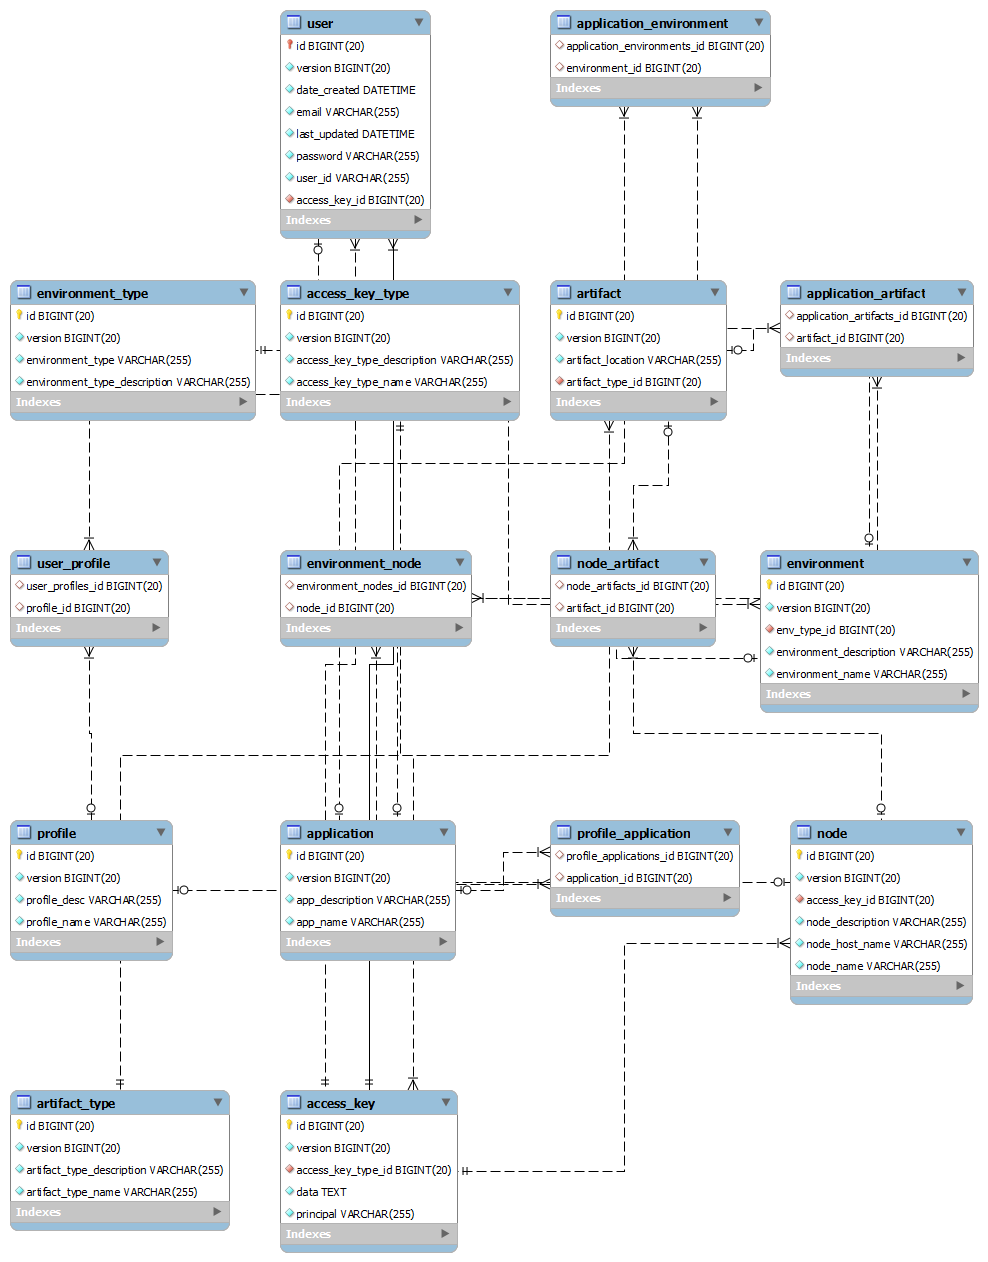
\includegraphics[scale=0.45]{ocelli.png}
    \caption{Ocelli Server Data Model}
    \label{fig:ocelli_dm}
\end{figure}

\section{Research Questions}

The research questions we are attempting to answer as part of this research paper are the following,

\begin{itemize}
\item Is it possible to build a completely passive machine generated data collector which can scale on all resources (cpu, network and memory) when centrally connected to, and reading data from a number of servers?
\item What is the impact such a system would have on the monitoring and monitored servers (cpu, memory) and on the network bandwidth between them.

Essentially, we wish to determine if a central server could provide the functionality required to support the real-time acquistation of data such that it can be examined and used by a human operator during an error event on any one of a large number of servers.
\end{itemize}

\section{Experimental Testbed}

In order to determine the viaibility of ingesting and processing data into a single server, tests will be performed using various instance types in Amazon's EC2 infrastructure [30]

\begin{itemize}
\item Virtualized network consisting of shared tenancy machines with 40 Mb to 1GB Networking
\item Virtualized network consisting of dedicated tenancy machines with 10GB Networking
\end{itemize}

\subsection{Simulation Environment}

\subsubsection{Amazon EC2}

The intial test environment consists an Ocelli Server, an Elastic Search server and 98 t2.micro [31] nodes, using Amazon's second generation T2 platform.

Specifications for the t2.micro are listed below

\begin{flushleft}
    \begin{tabular}{ | l | l |}
    \hline
  Attrubute & Value  \\ \hline
Max Network Bandwidth &  40 Mb/s	\\ \hline
CPU's &  1 vCpu	\\ \hline
Memory &  1 GB	\\ 
    \hline
    \end{tabular}
\end{flushleft}

\subsection{Simulation Approach and Setup}

Each test will consist of the following steps

\begin{itemize}
\item Load Ocelli Server Application UI
\item Select Application in Ocelli Server UI
\item Select Artifact to stream to Elastic Search
\item Begin Streaming
\end{itemize}

After these steps have been taken Ocelli Server will connect to every node containing the artifiact, begin reading from the end of the file, and then start pushing the data to the Elastic Search cluster. The data will then be available for inspection.

Ocelli will connect to each of the nodes and issue the following command
\\
\\
tail -f -c 1000000000 /logs/access.log
\\
\\
This will start a download of the last 1GB of the log file over ssh. 
\\
\\
The average line size in the log is 120 Bytes.

\subsubsection{Requirements and Test Setup}

The following are pre-requisites to performing a test run

\begin{itemize}
\item A User exists and is registered with Ocelli Server 
\item A User has a Profile Created
\item The User has added an Application to their Profile
\item All Nodes to be Monitored are registered with Ocelli Server (This will be performed via an SQL Script)
\item An Artifact exists on all Nodes and is registered with Ocelli Server (This will be performed via an SQL Script)
\item Each Artifact is a 1.6 GB Log File in /logs/access.log
\item The Elastic Search Cluster is empty and Indexes have been cleared
 \end{itemize}

\subsubsection{Key Analysis Areas}

There are certain metrics which will be recorded and monitored as each of the tests are run. The Ocelli Server itself (which is ingesting the data stream) will have its key metrics monitored, along with the nodes to which it is connected. Possible metrics to be monitored are listed below

\begin{itemize}
\item Average and Peak CPU Load on Ocelli Server
\item Average and Peak CPU Usage of Ocelli Java Server Process
\item Average and Peak CPU Usage of Elastic Search Server Process
\item Average and Peak Memory Usage on Ocelli Server
\item Average and Peak Memory Usage of Ocelli Java Server Process
\item Average and Peak Memory Usage of Elastic Search Server Process
\item Average and Peak Network Usage on Ocelli Server
\item Average and Peak Disk Usage on Ocelli Server
\item Average and Peak CPU Load on a Monitored Node
\item Average and Peak Memory Usage on a Monitored Node
\item Average and Peak Network Usage on a Monitored Node
\item Average and Peak Disk Usage on a Monitored Node
\end{itemize}

These metrics will be used to determine the performance of Ocelli Server and extrapolate the possibility of scaling the system further.

\subsection{Running the simulation}

\subsubsection{Application Setup}
The first step is to create the Application within the Ocelli Server UI, an example application is shown below\newline\newline
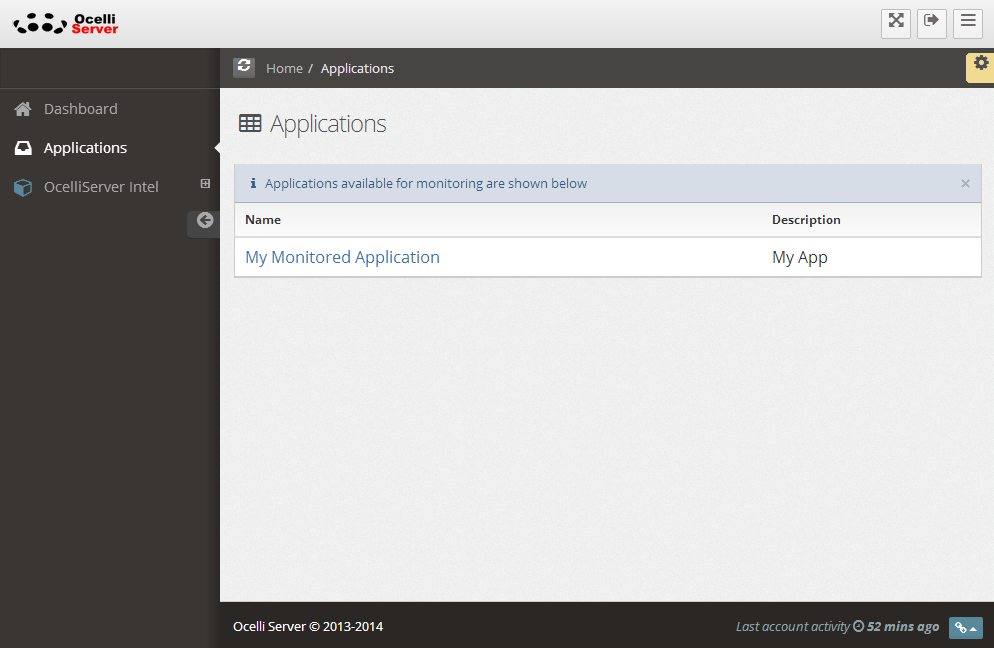
\includegraphics[scale=0.5]{app1}\newline\newline
\subsubsection{Streaming Setup}
Next, an Artifact must be selected for streaming to Elastic Search as show below, once the "Start Streaming" action has been confirmed in the Ocelli Server UI, data should begin streaming from the selected Artifact and appear in Elastic Search almost immediately. The Ocelli Server Java Application will connect via SSH to each of the servers one after another, so not all data will be streamed at once from each sever, rather it will graduallly increase.\newline\newline

For all of the tests the following will hold true

\begin{itemize}
\item /logs/access.log will be a single 1.6GB text file
\item Elastic Search will be installed and running on a seperate server to Ocelli Server
\item Each test will run for 5 minutes with a 5 minute warm up period occurring first
\end{itemize}

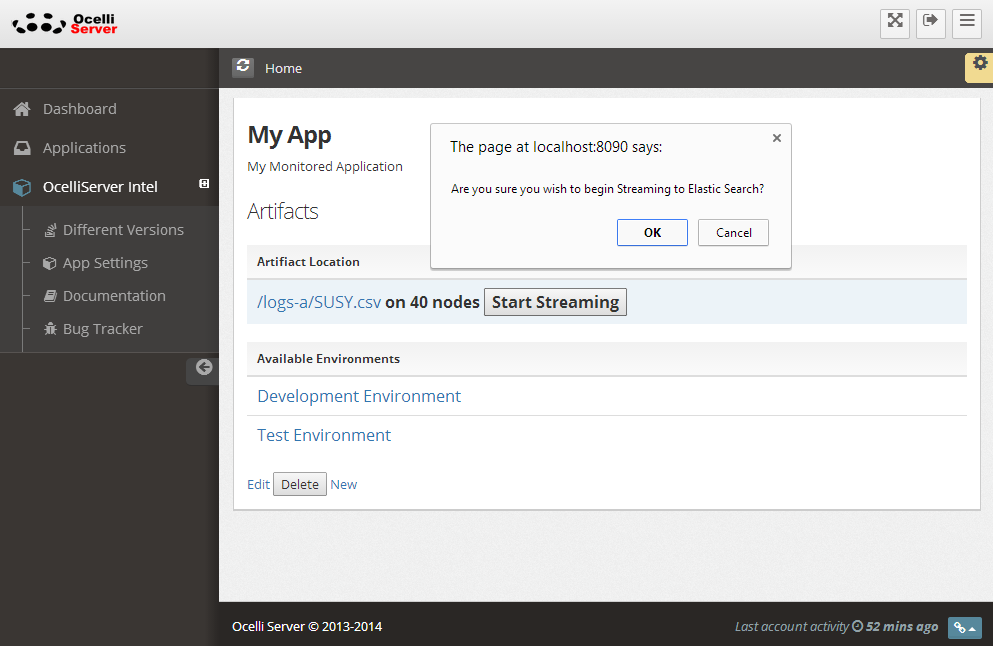
\includegraphics[scale=0.5]{app2}\newline\newline
There is also serverside setup for the simulation in the configuration of the Ocelli SSH Server. The ocelli.yml configuration file is modified to activate simulation mode and to add two additional variables, tpsCheckInterval and simulationRunTimeMillis\newline\newline
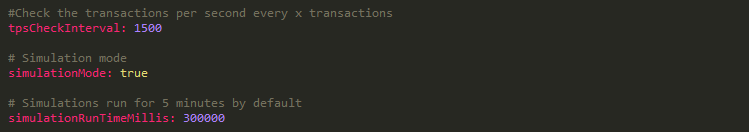
\includegraphics[scale=0.75]{app3}\newline\newline
tpsCheckInterval checks the number of transactions per second that Ocelli is able to process downstream to the ElasticSearch server, whilst simulationRunTimeMillis stops Ocelli from streaming after a certain amount of time has passed. This allows for timeboxed tests to be performed very easily.
\\
\\
Also, to warm up the JVM, the application is switched to "simulationMode: true" in ocelli.yml and the simulation is set to run for 5 minutes only. In the warm up phase Ocelli is also only connected connected to a single server on which it is streaming a single log from /logs/access.log.
\pagebreak
\section{Results and Analysis}
\subsection{Warmup}
During the warmup phase with Ocelli streaming from a single server the following results were observed in the application monitoring tool

\begin{figure}[h]
    \centering
    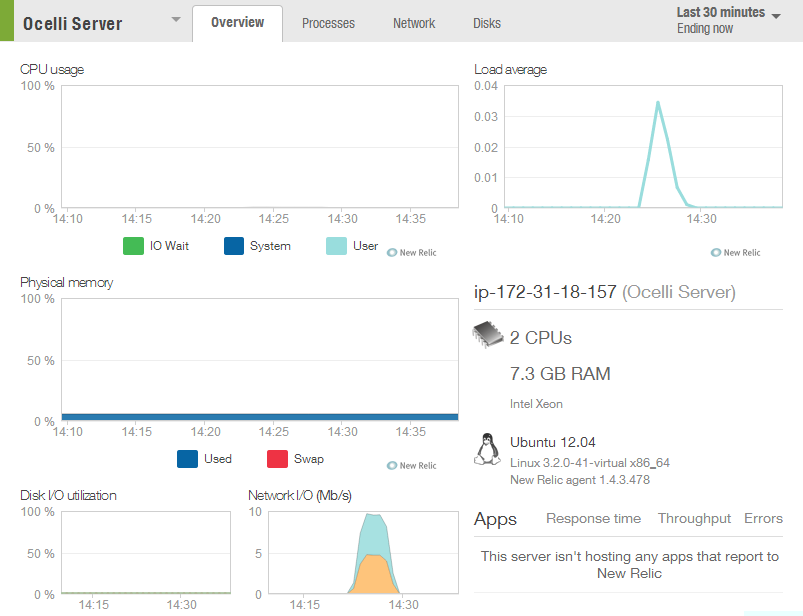
\includegraphics[scale=0.7]{app4}
    \caption{Ocelli Warm Up Results}
    \label{fig:ocelli_dm}
\end{figure}

The most taxed resource on the Ocelli Server was network bandwidth which peaked at 10Mbps, all other resource usages were nominal. Ocelli Server peaked at 819 tps (compared with 769 pre-warmup) and ingested 237,528 transactions to elasticsearch over exactly 300 seconds.

\begin{flushleft}
    \begin{tabular}{ | l | l |}
    \hline
  Attrubute & Value  \\ \hline
  Peak TPS & 819  \\ \hline
  Average and Peak CPU Load on Ocelli Server & 0.5\% / 6\%  \\ \hline
  Average and Peak CPU Usage of Ocelli Java Server Process & 0.3\% / 5.6\% \\ \hline
 Average and Peak CPU Usage of Elastic Search Server Process & 37.1\%/46.7\%	  \\ \hline
  Average and Peak Memory Usage on Ocelli Server & 400 MB / 426 MB	 \\ \hline
  Average and Peak Memory Usage of Ocelli Java Server Process &	200 MB / 210 MB		 \\ \hline
 Average and Peak Memory Usage of Elastic Search Server Process &	200 MB / 380 MB		 \\ \hline
Average and Peak Network Usage on Ocelli Server &	10 Mbps 	 \\ \hline
Peak Disk Usage on Ocelli Server &	2 IOPS (0.1\%) 		 \\ \hline
Average and Peak CPU Load on a Monitored Node& 	1\% 	 \\ \hline
  Average and Peak Memory Usage on a Monitored Node &	50MB / 55MB	 \\ \hline
Average and Peak Network Usage on a Monitored Node &	0.7 Mbps / 1.0 Mbps		 \\ \hline
  Average and Peak Disk Usage on a Monitored Node &  1\%	\\ 
    \hline
    \end{tabular}
\end{flushleft}

\subsection{Test 1 - 10 Servers}

During the next phase with Ocelli streaming from 10 app server instances the following results were observed in the application monitoring tool

\begin{figure}[h]
    \centering
    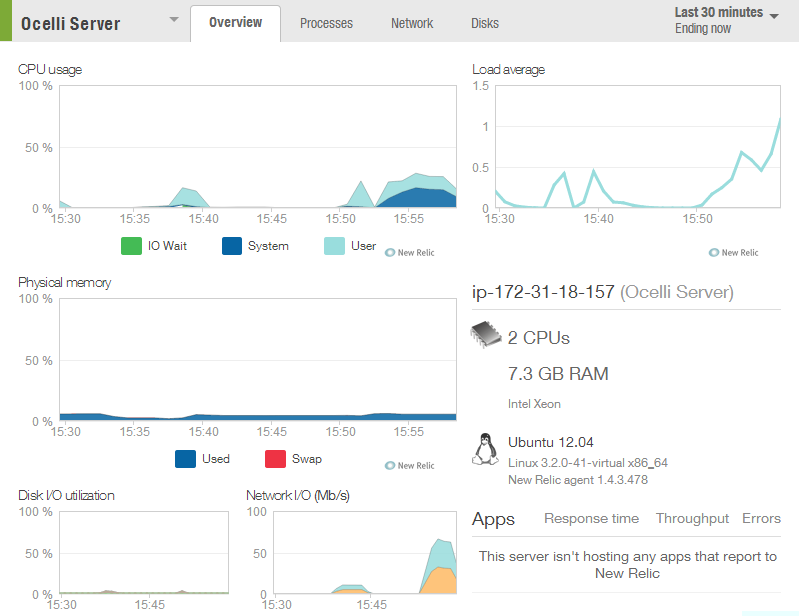
\includegraphics[scale=0.7]{app6}
    \caption{Ocelli Test 1 (10 Servers) - Results}
    \label{fig:ocelli_dm}
\end{figure}

The most taxed resource on the Ocelli Server was again, network bandwidth, which peaked at 65Mbps, all other resource usages were nomina except for CPU which started to rise to an average of 25\%. Ocelli Server peaked at 5084 tps (compared with 769 pre-warmup) and ingested 1,522,352 transactions to elasticsearch over exactly 300 seconds. At this point we can see that there are some key metrics that are starting to max out.

\begin{itemize}
\item CPU Usage of Elastic Search is now at 80.7\% Peak
\item Network Bandwidth for Ocelli Server is at 35 Mb/s Peak
\end{itemize}

\begin{flushleft}
    \begin{tabular}{ | l | l |}
    \hline
  Attrubute & Value  \\ \hline
  Peak TPS & 5084  \\ \hline
  Average and Peak CPU Load on Ocelli Server & 25\% / 50\%  \\ \hline
  Average and Peak CPU Usage of Ocelli Java Server Process & 20\% / 44.6\% \\ \hline
 Average and Peak CPU Usage of Elastic Search Server Process & 37.1\%/80.7\%	  \\ \hline
  Average and Peak Memory Usage on Ocelli Server & 410 MB / 416 MB	 \\ \hline
  Average and Peak Memory Usage of Ocelli Java Server Process &	244 MB / 250 MB		 \\ \hline
 Average and Peak Memory Usage of Elastic Search Server Process &	350 MB / 390 MB		 \\ \hline
Average and Peak Network Usage on Ocelli Server &	35 Mb/s 	 \\ \hline
Average and Peak Network Usage on Elastic Search Server & 25 Mb/s 	 \\ \hline
Peak Disk Usage on Ocelli Server &	2 IOPS (0.1\%)		 \\ \hline
Peak Disk Usage on Elastic Search Server &	80 IOPS (4.6\%)		 \\ \hline
Average and Peak CPU Load on a Monitored Node& 	1\% 	 \\ \hline
  Average and Peak Memory Usage on a Monitored Node &	50MB / 55MB	 \\ \hline
Average and Peak Network Usage on a Monitored Node &	0.7 Mbps / 1.0 Mbps		 \\ \hline
  Average and Peak Disk Usage on a Monitored Node &  1\%	\\ 
    \hline
    \end{tabular}
\end{flushleft}

One additional point of note was a slight delay in pickup from one of the SSH servers, which was roughly 10,000 transactions behind the rest of the streams. Once it was streaming, it kept up with the rest of the servers.

\subsection{Test 2 - 20 Servers and 98 Servers}

During the test at 20 servers it appears that we have reached the limit of the chosen instance trypes, from both a networking and CPU perspective. From the chart below we can see that we were unable to obtain any more bandwidth from Amazon between the first and second tests. Ocelli Server peaked at 5564 tps and ingested 1,635,360 transactions to elasticsearch over exactly 300 seconds

However, we were still bale to obtain a slight increase in peak TPS @ 5564 showing that doubling the amount of attached nodes still allows for an ingest rate of 278 transactions per server. This may still be enough to debug issues in real time during a crisis event. The slight increase can be attributed to further work performed by Elastic Search server which was not completely topped out on bandwith, allowing it to write additional transactions to disk, the increase in IOPS for Elastic Search shows it was still forced to make more writes in this test.

\begin{figure}[h]
    \centering
    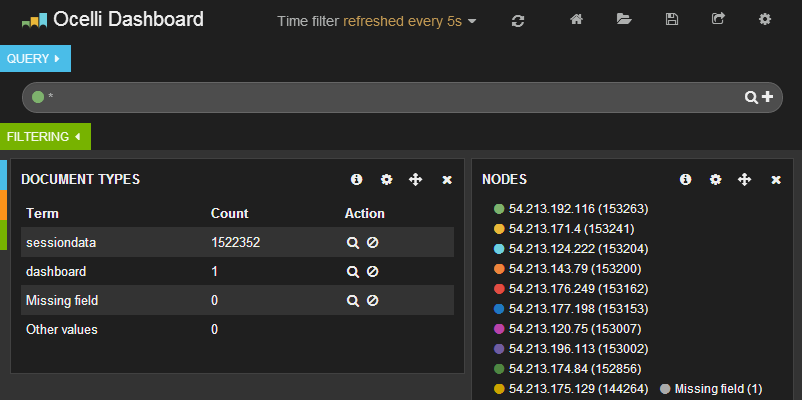
\includegraphics[scale=0.7]{app7}
    \caption{Ocelli Test 1 (Kibana dashboard showing server 53.213.175.129 fell behind)}
    \label{fig:ocelli_dm}
\end{figure}

\begin{figure}[h]
    \centering
    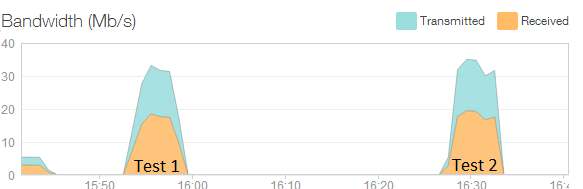
\includegraphics[scale=0.7]{app8}
    \caption{Comparison of network bandwidth for Ocelli Server between Test 1 and Test 2}
    \label{fig:ocelli_dm}
\end{figure}

\begin{flushleft}
    \begin{tabular}{ | l | l |}
    \hline
  Attrubute & Value  \\ \hline
  Peak TPS & 5564  \\ \hline
  Average and Peak CPU Load on Ocelli Server & 40\% / 50\%  \\ \hline
  Average and Peak CPU Usage of Ocelli Java Server Process & 30\% / 48.6\% \\ \hline
 Average and Peak CPU Usage of Elastic Search Server Process & 80.1\%/92.2\%	  \\ \hline
  Average and Peak Memory Usage on Ocelli Server & 410 MB / 416 MB	 \\ \hline
  Average and Peak Memory Usage of Ocelli Java Server Process &	300 MB / 300 MB		 \\ \hline
 Average and Peak Memory Usage of Elastic Search Server Process &	410 MB / 410 MB		 \\ \hline
Average and Peak Network Usage on Ocelli Server &	35 Mb/s 	 \\ \hline
Average and Peak Network Usage on Elastic Search Server & 26 Mb/s 	 \\ \hline
Peak Disk Usage on Ocelli Server &	2 IOPS (0.1\%)		 \\ \hline
Peak Disk Usage on Elastic Search Server &	114 IOPS (4.6\%)		 \\ \hline
Average and Peak CPU Load on a Monitored Node& 	1\% 	 \\ \hline
  Average and Peak Memory Usage on a Monitored Node &	50MB / 55MB	 \\ \hline
Average and Peak Network Usage on a Monitored Node &	0.7 Mbps / 1.0 Mbps		 \\ \hline
  Average and Peak Disk Usage on a Monitored Node &  1\%	\\ 
    \hline
    \end{tabular}
\end{flushleft}
\pagebreak
Before upgrading the Ocelli and Elastic Search servers, a test was performed at 98 nodes with the same configuration, Ocelli Server peaked at 5836 tps and ingested 1,750,863 transactions to elasticsearch over exactly 300 seconds. This is a 4\% performance improvement. One interesting result from this test was that although we did not manage to increase the throughput, the distribution of data collected per server was extremely even, to within +- 1\%. This means that there was no lag in connecting to the servers or collecting the data in the 98 node test, indicating that the outlier in Test 1 may have been just an anomaly. This can be seen below in Figure 6.

\begin{figure}[h]
    \centering
    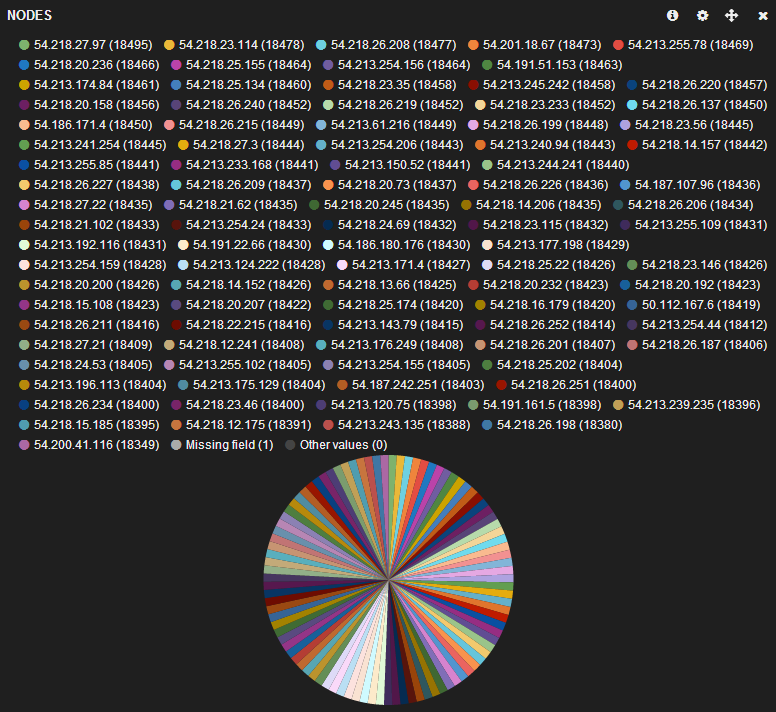
\includegraphics[scale=0.6]{app9}
    \caption{Kibana showing even distribution of data collected across nodes (~18.4k transactions per node)}
    \label{fig:ocelli_dm}
\end{figure}

However, we can see that we have completely exhausted the resources on the Elastic Search server and it cannot keep up with the data ingest.

\begin{figure}[h]
    \centering
    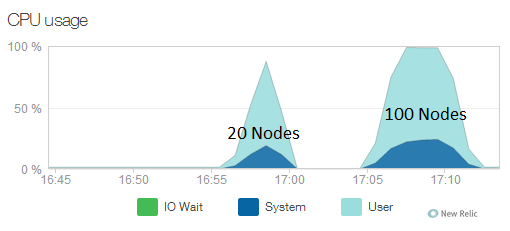
\includegraphics[scale=0.6]{app10}
    \caption{Elastic Search Server CPU ingesting data from 20 and 100 nodes respectively}
    \label{fig:ocelli_dm}
\end{figure}

\begin{figure}[h]
    \centering
    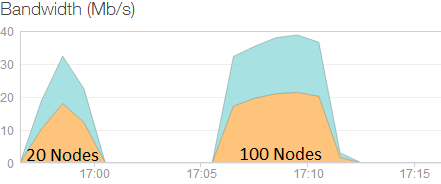
\includegraphics[scale=0.6]{app11}
    \caption{Network bandwidth usage at 20 and 100 nodes respectively for Ocelli Server}
    \label{fig:ocelli_dm}
\end{figure}

\begin{flushleft}
    \begin{tabular}{ | l | l |}
    \hline
  Attrubute & Value  \\ \hline
  Peak TPS & 5564  \\ \hline
  Average and Peak CPU Load on Ocelli Server &40\% / 60\%  \\ \hline
  Average and Peak CPU Usage of Ocelli Java Server Process & 39\% / 52.6\% \\ \hline
 Average and Peak CPU Usage of Elastic Search Server Process & 80.1\%/92.2\%	  \\ \hline
  Average and Peak Memory Usage on Ocelli Server & 1000 MB / 1050 MB	 \\ \hline
  Average and Peak Memory Usage of Ocelli Java Server Process &	855 MB / 860 MB		 \\ \hline
 Average and Peak Memory Usage of Elastic Search Server Process &	500 MB / 517 MB		 \\ \hline
Average and Peak Network Usage on Ocelli Server &	40 Mb/s 	 \\ \hline
Average and Peak Network Usage on Elastic Search Server & 30 Mb/s 	 \\ \hline
Peak Disk Usage on Ocelli Server &	2 IOPS (0.1\%)		 \\ \hline
Peak Disk Usage on Elastic Search Server &	107 IOPS (4.4\%)		 \\ \hline
Average and Peak CPU Load on a Monitored Node& 	1\% 	 \\ \hline
  Average and Peak Memory Usage on a Monitored Node &	50MB / 55MB	 \\ \hline
Average and Peak Network Usage on a Monitored Node &	0.7 Mbps / 1.0 Mbps		 \\ \hline
  Average and Peak Disk Usage on a Monitored Node &  1\%	\\ 
    \hline
    \end{tabular}
\end{flushleft}

At 100 nodes, we are at capacity with the following resources

\begin{itemize}
\item Ocelli Server Network Bandwidth - 100\% (40 Mb/s)
\item Elastic Search Server Network Bandwidth - 80\% (30 Mb/s)
\item Elastic Search Server CPU - 100\%
\end{itemize}

For the next test we will upgrade the Elastic Search Server so that it has more CPU and more network bandwidth.

\subsection{Test 3 - 98 Servers, Upgraded Elastic Search}

For this test, the Elastic Search Server is upgraded to a M3 General Purpose Double Extra Large (m3.2xlarge [31]), the specifications are show below

\begin{flushleft}
    \begin{tabular}{ | l | l |}
    \hline
  Attrubute & Value  \\ \hline
Max Network Bandwidth &  100 Mb/s	\\ \hline
CPU's &  8 Core (26 ECU)	\\ \hline
Memory &  30 GB	\\ 
    \hline
    \end{tabular}
\end{flushleft}

The results of this test are surprising, by upgrading the Elastic Search Server, we actually unlock a 2x increase in scale without upgrading the Ocelli Server. In fact, it seems that the Elastic Search server has been holding the Ocelli Server back. Ocelli Server peaked at 13163 tps and ingested 3,948,915 transactions to elasticsearch over exactly 300 seconds. This is a 136\% performance improvment from Test 2 at 98 nodes.

There are some interesting observations to made from this test.

Firtstly, even though the rated network throughput on the Ocelli Server is still 40 Mb/s, it manages to increase its through put for combined send and recieve to 83.5 MB/s. It is possible that this is due to the fact that it is now on an ingress network link of 100 Mb/s to the Elastic Search server, which is now at 100 MB/s and as such, can take advantage of that bandwith by the nature of being connected to that server. However, the addition of this bandwidth means that Ocelli Server is now using more CPU to push the data, and as such is beginning to also max out on CPU. For the next test, we will upgrade the Ocelli Server to an m3.2xlarge also. The Elastic search server itself is using about 40\% CPU on its new configuration. 

\begin{figure}[h]
    \centering
    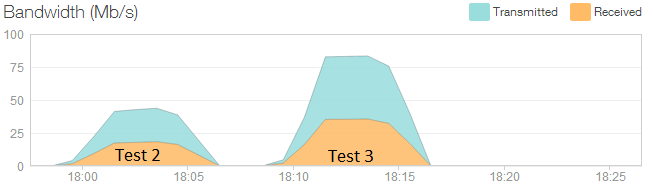
\includegraphics[scale=0.7]{app12}
    \caption{Network between test 2 and test 3 showing increased bandwidth availability for Ocelli Server}
    \label{fig:ocelli_dm}
\end{figure}

\begin{figure}[h]
    \centering
    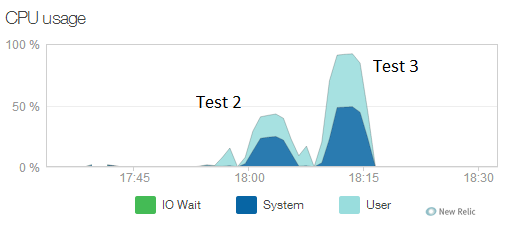
\includegraphics[scale=0.7]{app13}
    \caption{Ocelli Server nearing 100\% CPU utilization at 100 nodes for test 3}
    \label{fig:ocelli_dm}
\end{figure}

\begin{flushleft}
    \begin{tabular}{ | l | l |}
    \hline
  Attrubute & Value  \\ \hline
  Peak TPS & 5564  \\ \hline
  Average and Peak CPU Load on Ocelli Server &90\% / 90\%  \\ \hline
  Average and Peak CPU Usage of Ocelli Java Server Process & 92.0\% / 93.2\% \\ \hline
 Average and Peak CPU Usage of Elastic Search Server Process & 40.1\%/40.7\%	  \\ \hline
  Average and Peak Memory Usage on Ocelli Server & 1010 MB / 1020 MB	 \\ \hline
  Average and Peak Memory Usage of Ocelli Java Server Process &	855 MB / 870 MB		 \\ \hline
 Average and Peak Memory Usage of Elastic Search Server Process &	400 MB / 410 MB		 \\ \hline
Average and Peak Network Usage on Ocelli Server &	83.5 Mb/s 	 \\ \hline
Average and Peak Network Usage on Elastic Search Server & 62 Mb/s 	 \\ \hline
Peak Disk Usage on Ocelli Server &	2 IOPS (0.1\%)		 \\ \hline
Peak Disk Usage on Elastic Search Server &	145 IOPS (4.4\%)		 \\ \hline
Average and Peak CPU Load on a Monitored Node& 	1\% 	 \\ \hline
  Average and Peak Memory Usage on a Monitored Node &	50MB / 55MB	 \\ \hline
Average and Peak Network Usage on a Monitored Node &	0.7 Mbps / 1.0 Mbps		 \\ \hline
  Average and Peak Disk Usage on a Monitored Node &  1\%	\\ 
    \hline
    \end{tabular}
\end{flushleft}

\subsection{Test 4 - 98 Servers, Upgraded Ocelli Server}

For this test, the Ocelli Server is also upgraded to a M3 General Purpose Double Extra Large (m3.2xlarge [31])

During this test it is observed that although we have increased our throughput, Elastic Search has yet again become the bottle neck. Ocelli Server peaked at 22976 tps and ingested 6,893,024 transactions to elasticsearch over exactly 300 seconds. The Ocelli server read data at 144 Mb/s and sent to Elastic Search at 150 Mb/s, however Elastic search only reported ingesting at 74 Mb/s, with a combined network throughput of around 100 Mb/s as show below.

\begin{figure}[h]
    \centering
    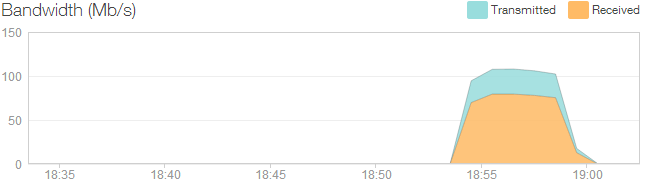
\includegraphics[scale=0.7]{app15}
    \caption{Elastic Search network bandwith chart showing 74 Mb/s ingress with 28.2 Mb/s transmitted}
    \label{fig:ocelli_dm}
\end{figure}

\begin{flushleft}
    \begin{tabular}{ | l | l |}
    \hline
  Attrubute & Value  \\ \hline
  Peak TPS & 22976  \\ \hline
  Average and Peak CPU Load on Ocelli Server &19\% / 20\%  \\ \hline
  Average and Peak CPU Usage of Ocelli Java Server Process & 16.0\% / 16.5\% \\ \hline
 Average and Peak CPU Usage of Elastic Search Server Process & 80.1\%/83.7\%	  \\ \hline
  Average and Peak Memory Usage on Ocelli Server & 1650 MB / 1670 MB	 \\ \hline
  Average and Peak Memory Usage of Ocelli Java Server Process &	1200 MB / 1200 MB		 \\ \hline
 Average and Peak Memory Usage of Elastic Search Server Process &	410 MB / 430 MB		 \\ \hline
Average and Peak Network Usage on Ocelli Server &	295.5 Mb/s 	 \\ \hline
Average and Peak Network Usage on Elastic Search Server & 108 Mb/s 	 \\ \hline
Peak Disk Usage on Ocelli Server &	2 IOPS (0.1\%)		 \\ \hline
Peak Disk Usage on Elastic Search Server &	159 IOPS (4.4\%)		 \\ \hline
Average and Peak CPU Load on a Monitored Node& 	1\% 	 \\ \hline
  Average and Peak Memory Usage on a Monitored Node &	50MB / 55MB	 \\ \hline
Average and Peak Network Usage on a Monitored Node &	0.7 Mbps / 1.0 Mbps		 \\ \hline
  Average and Peak Disk Usage on a Monitored Node &  1\%	\\ 
    \hline
    \end{tabular}
\end{flushleft}

\subsection{Test 5 - 98 Servers, Dedicated Hardware on 10GB Network for Ocelli Server and Elastic Search }

For this test, dedicated hardware was requested in AWS on c3.8xlarge [31] instances with 10GB networking for the Ocelli and the Elastic Search Server. The results of this test were deemed a failure as we could not obtain a performance improvement which was an order of magnitude greater (> 60\%) than Test 4. Ocelli Server peaked at 27562 tps and ingested 8,268,840 transactions to elasticsearch over exactly 300 seconds. This is an increase of only 19\% even though the hardware and networking have been drastically upgraded. Monitoring showed that networking was drastically underused. Total bandwidth used by ES was 138 Mb/s, only a 30 MB increase over Test 4 even though bandwidth is now 10GB/s (or 1000 MB/s). Ocelli Server Bandwidth stayed at 299 MB/s, only a 4 MB/s increase from non-dedicated hardware.

At this point, the t1.micro nodes containing the logs are analyzed, and it is determined that their network throughput may be actually the bottle neck as data cannot be pulled from them at greater than 500-700Kb/s. 

\begin{flushleft}
    \begin{tabular}{ | l | l |}
    \hline
  Attrubute & Value  \\ \hline
  Peak TPS & 27562  \\ \hline
  Average and Peak CPU Load on Ocelli Server &2\% / 3\%  \\ \hline
  Average and Peak CPU Usage of Ocelli Java Server Process & 2.0\% / 4.5\% \\ \hline
 Average and Peak CPU Usage of Elastic Search Server Process & 14.1\%/15.7\%	  \\ \hline
  Average and Peak Memory Usage on Ocelli Server & 2100 MB / 2100 MB	 \\ \hline
  Average and Peak Memory Usage of Ocelli Java Server Process &	2000 MB / 2000 MB		 \\ \hline
 Average and Peak Memory Usage of Elastic Search Server Process &	900 MB / 900 MB		 \\ \hline
Average and Peak Network Usage on Ocelli Server &	355.5 Mb/s 	 \\ \hline
Average and Peak Network Usage on Elastic Search Server & 122 Mb/s 	 \\ \hline
Peak Disk Usage on Ocelli Server &	2 IOPS (0.1\%)		 \\ \hline
Peak Disk Usage on Elastic Search Server &	190 IOPS (4.4\%)		 \\ \hline
Average and Peak CPU Load on a Monitored Node& 	1\% 	 \\ \hline
  Average and Peak Memory Usage on a Monitored Node &	50MB / 55MB	 \\ \hline
Average and Peak Network Usage on a Monitored Node &	0.7 Mbps / 1.0 Mbps		 \\ \hline
  Average and Peak Disk Usage on a Monitored Node &  1\%	\\ 
    \hline
    \end{tabular}
\end{flushleft}

After upgrading these to m3.medium class, Test 5 was rereun. The results of this test were also deemed a failure as we only achieved a performance increase of 37\%. However, Ocelli had an increased ingest bandwidth of 400 Mb/s suggesting that network bandwidth may have been the bottleneck. Ocelli Server peaked at 31614 tps and ingested 9,484,338 transactions to elasticsearch over exactly 300 seconds. The difference from the table above was negligible. The percentage increase is not enough to say that the m3.medium class servers made the difference.

At this point, it seems that it is not possible to increase the throughput of the system any further. Around 31,000 transactions per second is the maximum ingestion rate even when all bottlenecks have been removed. 

The only remaining area of examination is the performance of OpenSSH Server and the JSch java library itself.

\subsection{Test 6 - 98 Servers, HPN-SSH Server installed on App Servers}

HPN-SSH [32] is a variant of OpenSSH developed at the Pittsburg Super Computing Center. It patches OpenSSH in order to allow for tuning of internal flow control buffers. According to the documentation "These buffers often end up acting as a bottleneck for network throughput of SCP, especially on long and high bandwith network links. Modifying the ssh code to allow the buffers to be defined at run time eliminates this bottleneck".

openssh-6.6p1-hpnssh14v5 is installed on all of the app server nodes, and the following configuration is applied to each node at /etc/ssh d\_config

\begin{itemize}
\item TcpRcvBufPoll yes
\item \#NoneEnabled no
\item \#HPNDisabled no
\item HPNBufferSize 16384
\end{itemize}

The results of this test were deemed a success.  Ocelli Server peaked at 42,369 tps and ingested 12,710,760 transactions to elasticsearch over exactly 300 seconds. This is a 84\% increase from Test 4 and represents performance which comes close to doubling our scale.

Also it was noted that the installation of a more performant SSH library did not adversly affect resource usage on monitored nodes.

\begin{flushleft}
    \begin{tabular}{ | l | l |}
    \hline
  Attrubute & Value  \\ \hline
  Peak TPS & 42369  \\ \hline
  Average and Peak CPU Load on Ocelli Server &3\% / 4\%  \\ \hline
  Average and Peak CPU Usage of Ocelli Java Server Process & 2.0\% / 3.5\% \\ \hline
 Average and Peak CPU Usage of Elastic Search Server Process & 15.1\%/15.7\%	  \\ \hline
  Average and Peak Memory Usage on Ocelli Server & 3450 MB / 3450 MB	 \\ \hline
  Average and Peak Memory Usage of Ocelli Java Server Process &	3000 MB / 3000 MB		 \\ \hline
 Average and Peak Memory Usage of Elastic Search Server Process &	1360 MB / 1360 MB		 \\ \hline
Average and Peak Network Usage on Ocelli Server &	295.5 Mb/s 	 \\ \hline
Average and Peak Network Usage on Elastic Search Server & 210 Mb/s 	 \\ \hline
Peak Disk Usage on Ocelli Server &	2 IOPS (0.1\%)		 \\ \hline
Peak Disk Usage on Elastic Search Server &	322 IOPS (4.4\%)		 \\ \hline
Average and Peak CPU Load on a Monitored Node& 	1\% 	 \\ \hline
  Average and Peak Memory Usage on a Monitored Node &	50MB / 55MB	 \\ \hline
Average and Peak Network Usage on a Monitored Node &	0.7 Mbps / 1.5 Mbps		 \\ \hline
  Average and Peak Disk Usage on a Monitored Node &  1\%	\\ 
    \hline
    \end{tabular}
\end{flushleft}

\section{Summary and Conclusions}

The data obtained from running these simulations shows that indeed, it is possible to ingest data from a large number of servers into a single machine whilst maintaing performance across all nodes. The bottleneck for these simulations started out with CPU and networking, but once servers were upgraded, it becomes clear that the actual bottleneck are components within the SSH stack we are using. During the final test each node had data extracted at around 0.9 Mb/s to 1.5 Mb/s, an increase from all previous tests, showing that HPN-SSH was able to increase the throughput significantly. 

The bandwidth for the final test on the Ocelli Server is 10 GB/s, meaning each of the 98 connected nodes has a theoretical maximum throughput of 10.2 MB/s into Ocelli Server. However, each node only achieves less than 10\% of its potential. This is due to the fact that Ocelli can not pull from each server at greater than 1.5 MB/s, indicating that it is in fact the SSH Server and/or SSH library which is causing the problem.

In the final test, a global TPS of 42,369 at 98 nodes (M\textsubscript{nodes}) indicated that we achieved a global 432 TPS per server (G\textsubscript{tps}). This is a drop of 48\% from our single server simulation in Test 1 (O\textsubscript{tps}) indicating that each server introduces a 0.49\% overhead or reduces G\textsubscript{tps} by 3.94 (C\textsubscript{loss}). Using the conditions in Test 6, the theoretical maximum amount of servers (S\textsubscript{cap}) that could be supported by this configuration, whilst still allowing for 29 TPS (R\textsubscript{tps}) per server would be an additional 102 servers, for a total of 200. The formula for this calculation is below
\\
\begin{align}
\dfrac{ (G\textsubscript{tps} - R\textsubscript{tps}) / C\textsubscript{loss}}{ (O\textsubscript{tps} - G\textsubscript{tps}) / M\textsubscript{nodes}} = S\textsubscript{cap}
\end{align}

In order to improve throughput, we must find a method with which to expand the throughput obtained from each app server node. As we know there are no longer any networking bottlenecks, there are 4 theories as to why performance dropped off, even with improved networking

\begin{itemize}
\item 
\item The 'tail' command is unable to deliver data to the OpenSSH server faster than 1.5 MB/s
\item The OpenSSH server is unable to allow download speeds of greater than 1.5 MB/s
\item The JSch client is unable to download data at faster than 1.5 MB/s
\item The Ocelli Server usage of the JSch client is inefficient
\end{itemize}

A quick test using
\\
\\
tail -f -c 1000000000 /logs/access.log \textgreater  test2.log
\\
\\
shows that the 1GB is written in 25 seconds, or 40MB/s on a t2.micro instance, so the issue is clearly with OpenSSH Server or JSch. Extending this to a quick remote test shows that when the same file is downloaded via the standard SSH client on the Ocelli Server, the transfer is much faster :
\\
\\
ssh -i app.pem ec2-user@server  "tail -f -c 1000000000 /logs/access.log" \textgreater  test2.log
\\
\\
The above comand produces a 1GB file on the Ocelli Server in 48 seconds, or 20 MB/s. It is therefore conclusive that it is either the JSch library itself, or Ocelli's Server's usage of the library that is the source of the performance issue. As such, further research could be conducted to improve transfer rates within the library for standard SSH connections. It is possible that a standard SCP command from JSch would improve performance, however this would be outside of the scope of this paper, and would only allow for the download of the file at regular intervals, therefore stifling the real time aspect of the research. It is also possible that tuning the I/O read buffer in Ocelli Server could provide some performance boosts although time was not available to test this scenario.

\pagebreak
\begin{thebibliography}{}  % (do not forget {})
\bibitem{bib:one_book}8+ Splunk Alternatives | DevOpsANGLE. [online] Available at: \textless http://devopsangle.com/2012/04/19/8-splunk-alternatives/\textgreater [Accessed 1 Sep. 2014].
\bibitem{bib:one_book}Build your own profiling tool. [online] Available at: \textless http://www.ibm.com/developerworks/library/j-jip/\textgreater [Accessed 1 Sep. 2014].
\bibitem{bib:one_book}CouchDB for access log aggregation and analysis - User Primary. [online] Available at: \textless http://userprimary.net/posts/2009/06/13/couchdb-for-access-log-aggregation-and-analysis/\textgreater [Accessed 1 Sep. 2014].
\bibitem{bib:one_book}CUED SSH2 - how to use it. [online] Available at: \textless http://www-h.eng.cam.ac.uk/help/jpmg/SSH2/adv-use.html\#compress\textgreater [Accessed 1 Sep. 2014].
\bibitem{bib:one_book}Enterprise Information Management Software EIM | Technology | SAP. [online] Available at: \textless http://www54.sap.com/solutions/tech/enterprise-information-management.html\textgreater [Accessed 1 Sep. 2014].
\bibitem{bib:one_book}Hierarchical In-Network Data Aggregation with Quality Guarantees - Springer. [online] Available at: \textless http://link.springer.com/chapter/10.1007\%2F978-3-540-24741-8\_38?LI=true\textgreater [Accessed 1 Sep. 2014].
\bibitem{bib:one_book}Java Concurrency (\&c): Profiling with JVMTI/JVMPI, SIGPROF and AsyncGetCallTrace. [online] Available at: \textless http://jeremymanson.blogspot.com/2007/05/profiling-with-jvmtijvmpi-sigprof-and.html\textgreater [Accessed 1 Sep. 2014].
\bibitem{bib:one_book} Java Tip 92: Use the JVM Profiler Interface for accurate timing - JavaWorld. [online] Available at: \textless http://www.javaworld.com/javaworld/javatips/jw-javatip92.html?page=2\textgreater [Accessed 1 Sep. 2014].
\bibitem{bib:one_book}JSTOR: The American Economic Review, Vol. 58, No. 4 (Sep., 1968), pp. 773-787. [online] Available at: \textless http://www.jstor.org/discover/10.2307/1815532?uid=3739696\textgreater [Accessed 1 Sep. 2014].
\bibitem{bib:one_book}Machine-generated data - Wikipedia, the free encyclopedia. [online] Available at: \textless http://en.wikipedia.org/wiki/Machine-generated\_data\textgreater [Accessed 1 Sep. 2014].
\bibitem{bib:one_book} Matt Casters on Data Integration » Real-time streaming data aggregation. [online] Available at:
\textless http://www.ibridge.be/?p=204\textgreater [Accessed 1 Sep. 2014].
\bibitem{bib:one_book}Splunking the JVM (Java Virtual Machine). [online] Available at: \textless http://www.slideshare.net/damiendallimore/splunking-the-jvm-java-virtual-machine\#btnNext\textgreater [Accessed 1 Sep. 2014].
\bibitem{bib:one_book} syslog - Splunk is fantastically expensive: What are the alternatives? - Server Fault. [online] Available at: \textless http://serverfault.com/questions/239401/splunk-is-fantastically-expensive-what-are-the-alternatives\textgreater [Accessed 1 Sep. 2014].
\bibitem{bib:one_book} valz - Scalable and robust distributed data aggregation, as easy as logging - Google Project Hosting. [online] Available at: \textless http://code.google.com/p/valz/\textgreater [Accessed 1 Sep. 2014].
\bibitem{bib:one_book}Wireless sensor network - Wikipedia, the free encyclopedia. [online] Available at: \textless http://en.wikipedia.org/wiki/Wireless\_sensor\_network\textgreater [Accessed 1 Sep. 2014].
\bibitem{bib:one_book} Examples of machine-generated data | DBMS 2 : DataBase Management System Services. [online] Available at: \textless http://www.dbms2.com/2010/04/08/machine-generated-data-example/\textgreater [Accessed 1 Sep. 2014].
\bibitem{bib:one_book} Examples and definition of machine-generated data | DBMS 2 : DataBase Management System Services. [online] Available at: \textless http://www.dbms2.com/2010/12/30/examples-and-definition-of-machine-generated-data/\textgreater [Accessed 1 Sep. 2014].
\bibitem{bib:one_book} Page 10 - Chromium Renderserver: Scalable and Open Source Remote Rendering Infrastructure [eScholarship]. [online] Available at: \textless http://escholarship.ucop.edu/uc/item/08t699fr\textgreater [Accessed 1 Sep. 2014].
\bibitem{bib:one_book} JSch - Java Secure Channel. [online] Available at: \textless http://www.jcraft.com/jsch/\textgreater [Accessed 1 Sep. 2014].
\bibitem{bib:one_book} The Java Virtual Machine Profiler Interface | Dr Dobb’s. [online] Available at: \textless http://www.drdobbs.com/jvm/the-java-virtual-machine-profiler-interf/184405722\textgreater [Accessed 1 Sep. 2014].
\bibitem{bib:one_book} The Java Virtual Machine Profiler Interface (JVMPI). [online] Available at: \textless http://docs.oracle.com/javase/1.4.2/docs/guide/jvmpi/jvmpi.html\textgreater [Accessed 1 Sep. 2014].
\bibitem{bib:one_book} Bloom Filters by Example. [online] Available at: \textless http://billmill.org/bloomfilter-tutorial/\textgreater [Accessed 1 Sep. 2014].
\bibitem{bib:one_book} View the latest version that the requested documentation is available in. - Splunk Knowledgebase. [online] Available at:
\textless http://docs.splunk.com/Special:SpecialLatestDoc?t=Documentation/Splunk/latest/Admin/Bloomfilters\textgreater [Accessed 1 Sep. 2014].
\bibitem{bib:one_book} Splunk Breakthrough Recognized with Grant of U.S. Patent for Organizing and Understanding Massive Machine Data. [online] Available at: \textless http://www.splunk.com/view/SP-CAAAF8J\textgreater [Accessed 1 Sep. 2014].
\bibitem{bib:one_book} Platform Monitoring and Management Using JMX. [online] Available at: \textless http://docs.oracle.com/javase/1.5.0/docs/guide/management/agent.html\textgreater [Accessed 1 Sep. 2014].
\bibitem{bib:one_book} JDK 5.0 Java Virtual Machine Tool Interface (JVMTI)-related APIs \& Developer Guides -- from Sun Microsystems. [online] Available at: \textless http://docs.oracle.com/javase/1.5.0/docs/guide/jvmti/\textgreater [Accessed 1 Sep. 2014].
\bibitem{bib:one_book} Enterprise information management - Wikipedia, the free encyclopedia. [online] Available at: \textless http://en.wikipedia.org/wiki/Enterprise\_information\_management\textgreater [Accessed 1 Sep. 2014].
\bibitem{bib:one_book} Enterprise Information Management Software EIM | Technology | SAP. [online] Available at: \textless http://www54.sap.com/solutions/tech/enterprise-information-management.html\textgreater [Accessed 1 Sep. 2014].
\bibitem{bib:one_book}Elasticsearch.org Open Source Distributed Real Time Search \& Analytics | Elasticsearch. [online] Available at: <http://www.elasticsearch.org/> [Accessed 1 Sep. 2014].
\bibitem{bib:one_book}AWS | Amazon Elastic Compute Cloud (EC2) - Scalable Cloud Hosting. [online] Available at: <http://aws.amazon.com/ec2/> [Accessed 1 Sep. 2014].
\bibitem{bib:one_book}AWS | Amazon EC2 | Instance Types. [online] Available at: <http://aws.amazon.com/ec2/instance-types/> [Accessed 1 Sep. 2014].
\bibitem{bib:one_book}HPN-SSH. [online] Available at: <http://www.psc.edu/index.php/hpn-ssh> [Accessed 1 Sep. 2014].

\end{thebibliography}
%
\end{document}
